Infine, studiamo i \textit{diagrammi di attività} (detti anche \textit{Activity Diagram}). \\
Questi vengono utilizzati per descrivere le singole fasi dei processi interni più complessi. Nel nostro scenario, l'activity diagram modellerà il comportamento del sistema attraverso molteplici contesti operativi. Per rendere l'analisi più chiara e strutturata, ho deciso di suddividere la modellazione dei flussi di lavoro in base ai principali attori che interagiscono con la piattaforma e ai moduli di sistema più critici.

% SEZIONE UTENTE REGISTRATO

\subsection*{Azioni dell'Utente Registrato}
Il primo attore preso in esame è l'Utente Registrato. \\ Questo attore, è colui che andrà ad usare il software frequentemente per i propri spostamenti quotidiani. \\
Il suo ingresso nel sistema è regolato dal flusso di autenticazione e recupero credenziali, modellato in Figura \ref{fig:ur_auth}.

\begin{figure}[H]
    \centering
    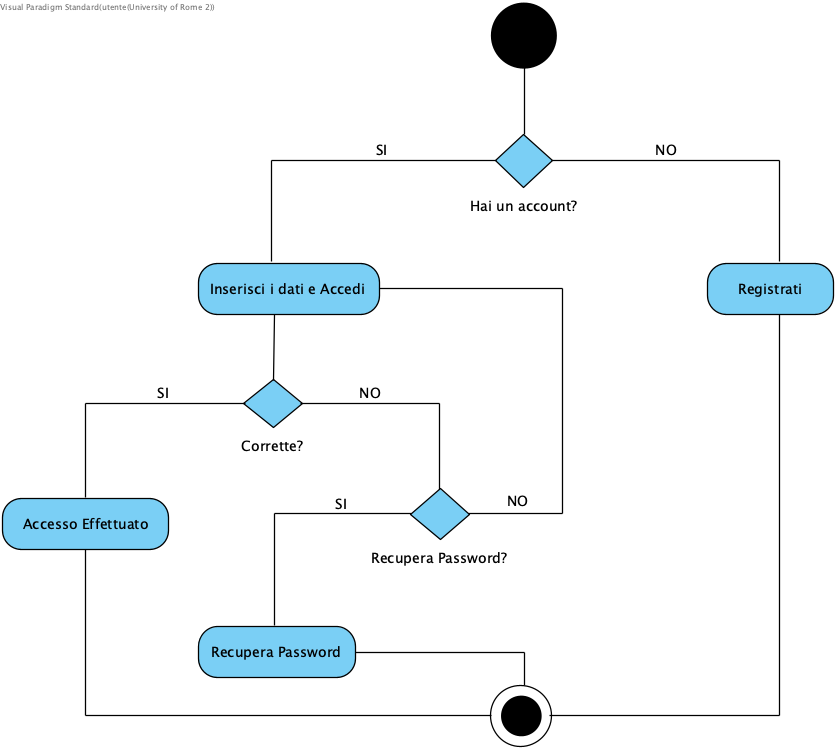
\includegraphics[width=0.8\textwidth]{Activity Diagram/Utente_Registrato/Utente_Registrato_(Autenticazione).png}
    \caption{}
    \label{fig:ur_auth}
\end{figure}
\vspace{1em}
\noindent
Una delle operazioni più frequenti compiute da questo utente è la ricerca di percorsi. \\ Accedendo al portale, egli può inserire i parametri di viaggio desiderati e avviare una ricerca iterativa fino all'individuazione di una soluzione valida (Figura \ref{fig:ur_mobilita}). A supporto di questa funzionalità, ho inserito una logica di salvataggio (Figura \ref{fig:ur_preferiti}): l'utente può aggiungere o rimuovere le tratte abituali nell'area Preferiti, migliorando notevolmente l'usabilità del software.
\begin{figure}[H]
    \centering
    \begin{minipage}{0.3\textwidth}
        \centering
        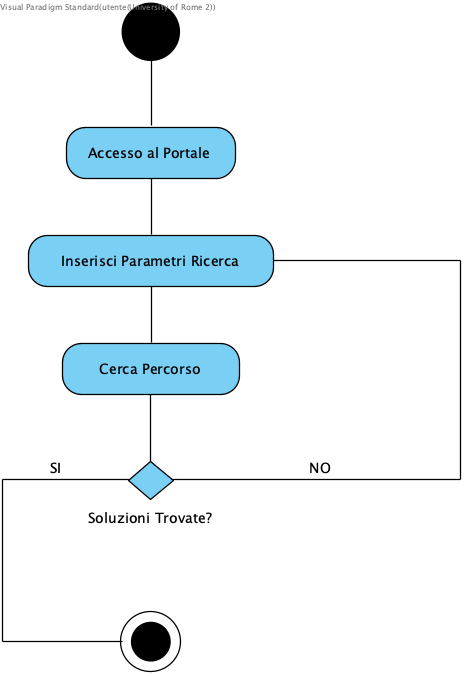
\includegraphics[width=\textwidth]{Activity Diagram/Utente_Registrato/Utente_Registrato_(Consulta MObilità).png}
        \caption{}
        \label{fig:ur_mobilita}
    \end{minipage}\hfill
    \begin{minipage}{0.6\textwidth}
        \centering
        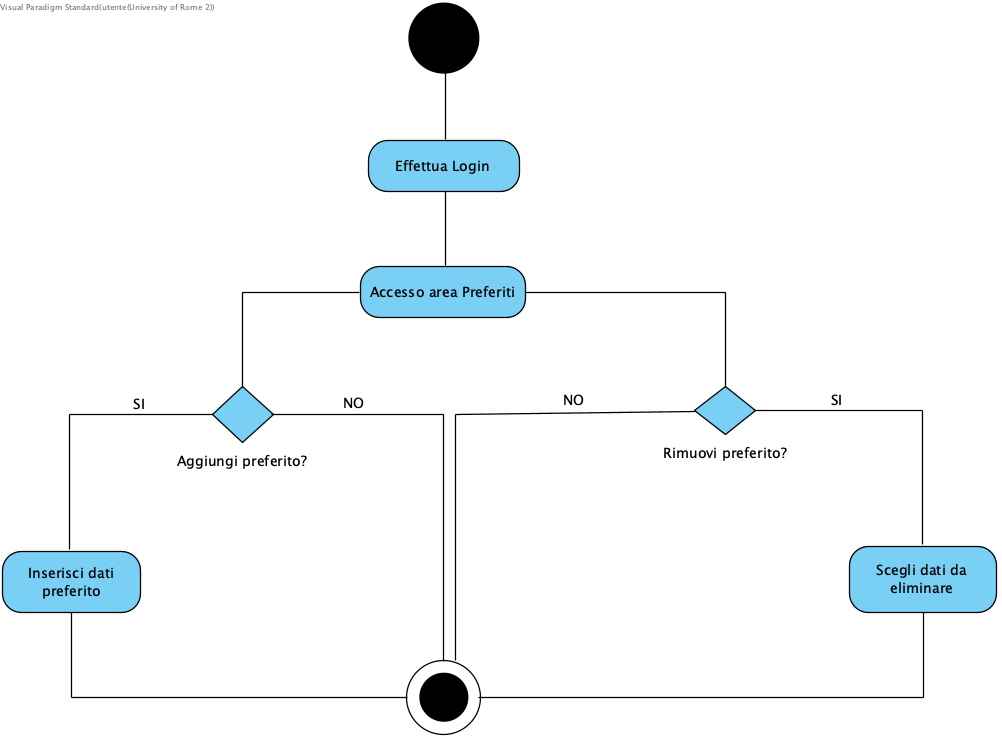
\includegraphics[width=\textwidth]{Activity Diagram/Utente_Registrato/Utente_Registarto_(Gestione_Preferiti).png}
        \caption{}
        \label{fig:ur_preferiti}
    \end{minipage}
\end{figure}
\noindent
L'applicativo gestisce in modo fluido anche i pagamenti per la sosta e il trasporto. \\ Nei diagrammi \ref{fig:ur_pag_biglietto} e \ref{fig:ur_pag_sosta} ho analizzato due scenari di acquisto molto simili ma concettualmente separati: l'acquisto di un normale biglietto (selezionando il titolo, i dati e il metodo di pagamento) e il pagamento per la sosta del proprio veicolo.
\begin{figure}[H]
    \centering
    \begin{minipage}{0.35\textwidth}
        \centering
        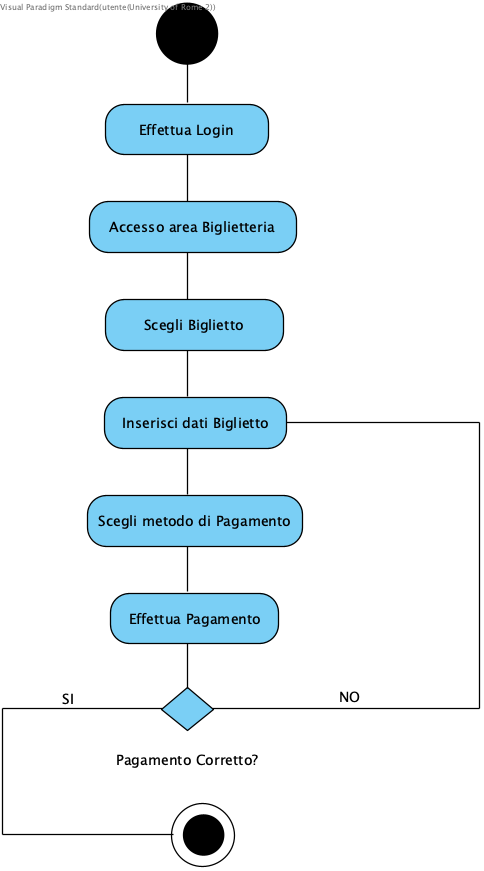
\includegraphics[width=\textwidth]{Activity Diagram/Utente_Registrato/Utente_Registrato_(Pagamento_Biglietto).png}
        \caption{}
        \label{fig:ur_pag_biglietto}
    \end{minipage}\hfill
    \begin{minipage}{0.35\textwidth}
        \centering
        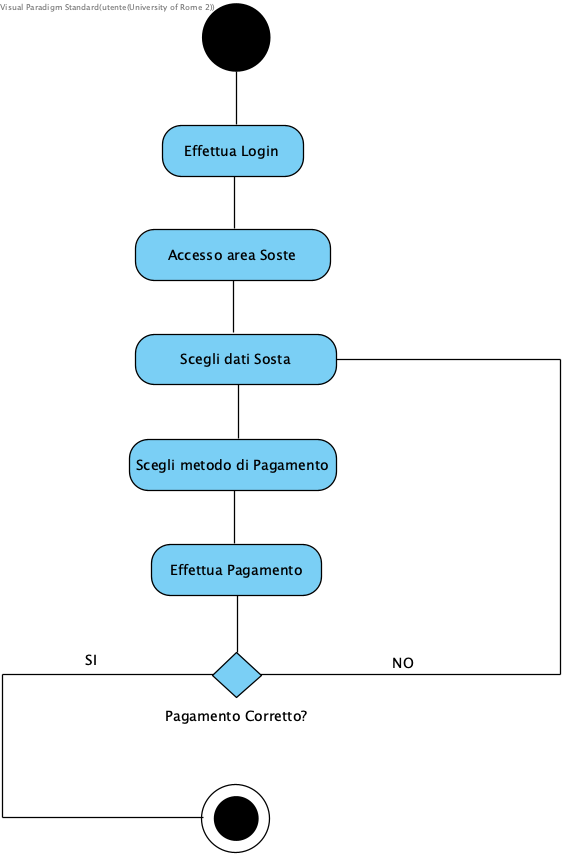
\includegraphics[width=\textwidth]{Activity Diagram/Utente_Registrato/Utente_Registrato_(Pagamento_Sosta).png}
        \caption{}
        \label{fig:ur_pag_sosta}
    \end{minipage}
\end{figure}
\noindent
Un'altra caratteristica, innovativa e molto importante che ha un impatto positivo sull'ambiente, è la prenotazione del servizio DRT (Trasporto a Chiamata). Come evidenziato in Figura \ref{fig:ur_drt}, dopo aver inserito i parametri e trovato una soluzione compatibile, l'utente seleziona le opzioni ed effettua la chiamata effettiva verso l'operatore.
\begin{figure}[H]
    \centering
    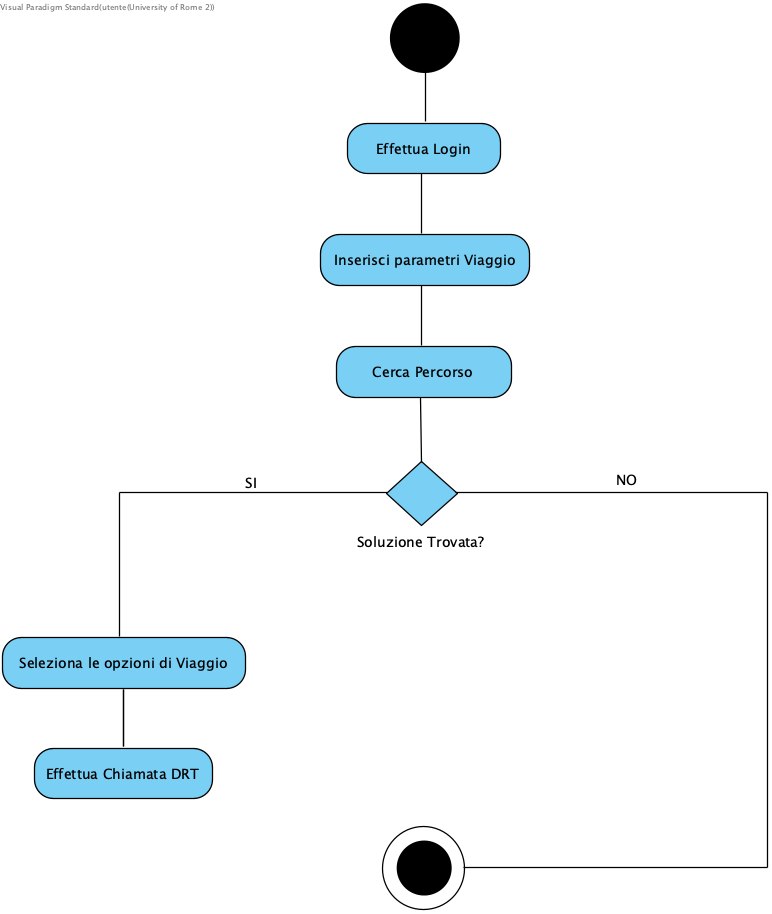
\includegraphics[width=0.45\textwidth]{Activity Diagram/Utente_Registrato/Utente_Registrato_(Prenotazione_DRT).png}
    \caption{}
    \label{fig:ur_drt}
\end{figure}
\noindent
Per concludere l'analisi di questo attore, ho modellato in Figura \ref{fig:ur_storico} la consultazione dello storico: accedendo all'area Cronologia, l'utente ha la possibilità di avere un resoconto chiaro e immediato di tutti i propri viaggi passati.
\begin{figure}[H]
    \centering
    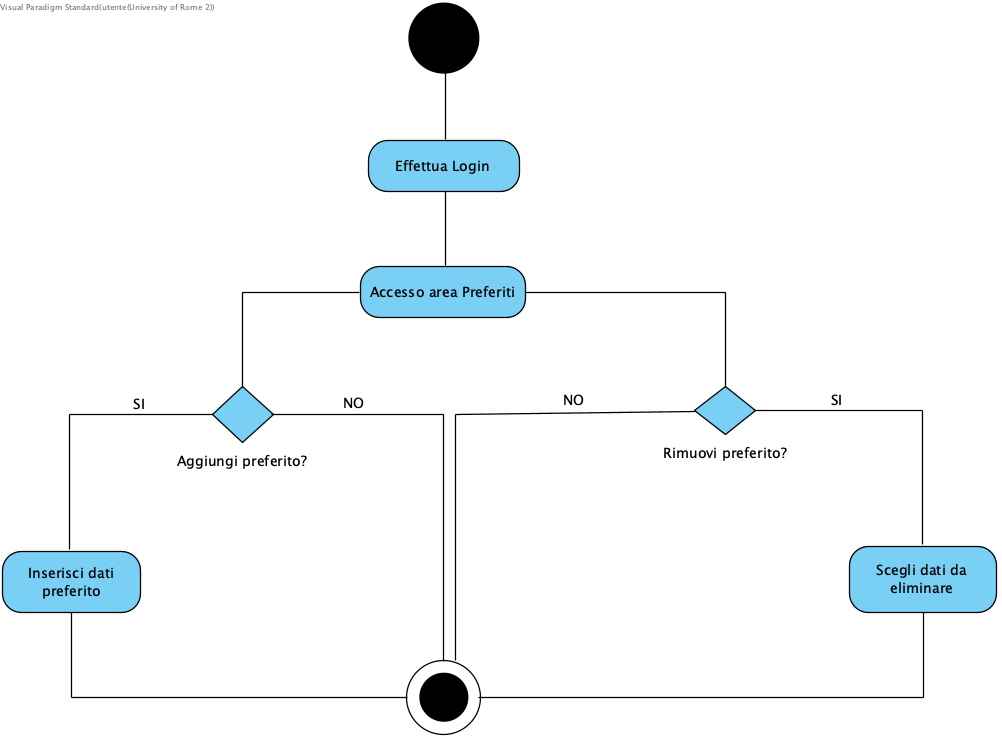
\includegraphics[width=0.6\textwidth]{Activity Diagram/Utente_Registrato/Utente_Registarto_(Gestione_Preferiti).png}
    \caption{}
    \label{fig:ur_storico}
\end{figure}

\newpage
% SEZIONE UTENTE NON REGISTRATO
\subsection*{Azioni dell'Utente Non Registrato}
A seguire, ho ritenuto opportuno descrivere anche il comportamento dell'utente il quale naviga sulla piattaforma senza possedere un account. \\
L'utente non registrato ha un accesso limitato, ma può comunque usufruire di alcune funzionalità per disporre in parte del servizio, come la consultazione della mobilità. \\ Come illustrato in Figura \ref{fig:unreg_mobilita}, il visitatore accede al portale, inserisce i parametri di ricerca e il sistema valuta iterativamente se esistono soluzioni di viaggio conformi ai criteri immessi.
\begin{figure}[H]
    \centering
    \includegraphics[width=0.25\textwidth]{Activity Diagram/Utente_non_Registrato/Utente_non_Registrato_(Consulta MObilità) copia.png}
    \caption{}
    \label{fig:unreg_mobilita}
\end{figure}
\noindent
Qualora l'utente decidesse di voler sfruttare tutte le potenzialità del sistema può attivare il processo di registrazione (Figura \ref{fig:unreg_registrazione}). Il flusso prevede la compilazione di un form e un ciclo di verifica fino alla corretta sottomissione dei dati.
\begin{figure}[H]
    \centering
    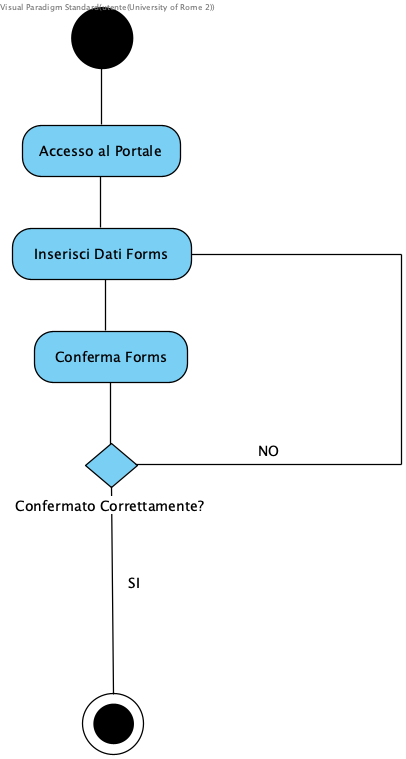
\includegraphics[width=0.25\textwidth]{Activity Diagram/Utente_non_Registrato/Utente_non_Registrato_(Registrazione).png}
    \caption{}
    \label{fig:unreg_registrazione}
\end{figure}
\newpage
% SEZIONE TURISTA
\subsection*{Azioni del Turista}
L'ultimo attore che usa il software come "consumatore" è il Turista. \\ Una volta effettuato l'accesso, l'interesse principale di questo attore è esplorare l'offerta di mobilità dedicata e acquistare i titoli di viaggio. Il flusso di consultazione è estremamente lineare: come mostrato in Figura \ref{fig:turista_consultazione}, l'utente accede all'area biglietteria ed esamina i pacchetti speciali disponibili.
\begin{figure}[H]
    \centering
    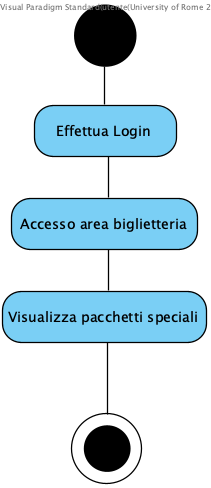
\includegraphics[width=0.2\textwidth]{Activity Diagram/Turista/Turista_(Consultazione_pacchetti).png}
    \caption{}
    \label{fig:turista_consultazione}
\end{figure}
\vspace{1em}
\noindent
Se il turista decide di procedere con l'acquisto di un pacchetto, il diagramma di attività si espande (Figura \ref{fig:turista_acquisto}). Dopo aver selezionato il pacchetto di interesse, l'utente procede all'inserimento dei dati di fatturazione fino al raggiungimento di un esito positivo della transazione.
\begin{figure}[H]
    \centering
    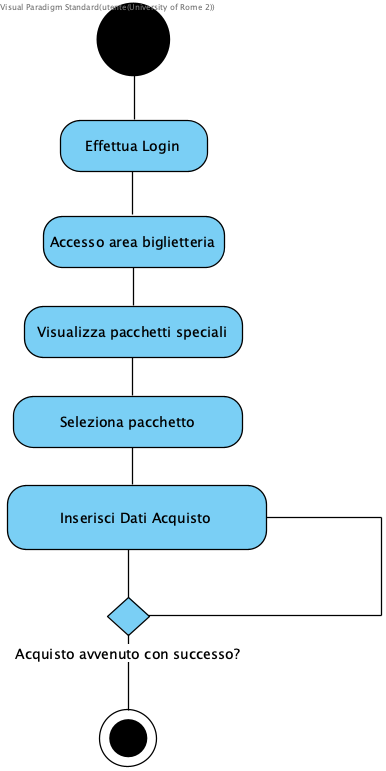
\includegraphics[width=0.25\textwidth]{Activity Diagram/Turista/Turista_(Acquista_Pacchetti).png}
    \caption{}
    \label{fig:turista_acquisto}
\end{figure}
\newpage
% SEZIONE ADMIN ENTE
\subsection*{Azioni dell'Admin Ente}
Spostandoci ora sul lato gestionale della piattaforma, analizziamo l'Admin dell'Ente. \\ Come per ogni utente del sistema, il primo passo fondamentale è l'autenticazione. Il diagramma in Figura \ref{fig:admin_auth} mostra il flusso decisionale che porta al login, alla registrazione o al recupero della password in caso di credenziali errate.
\begin{figure}[H]
    \centering
    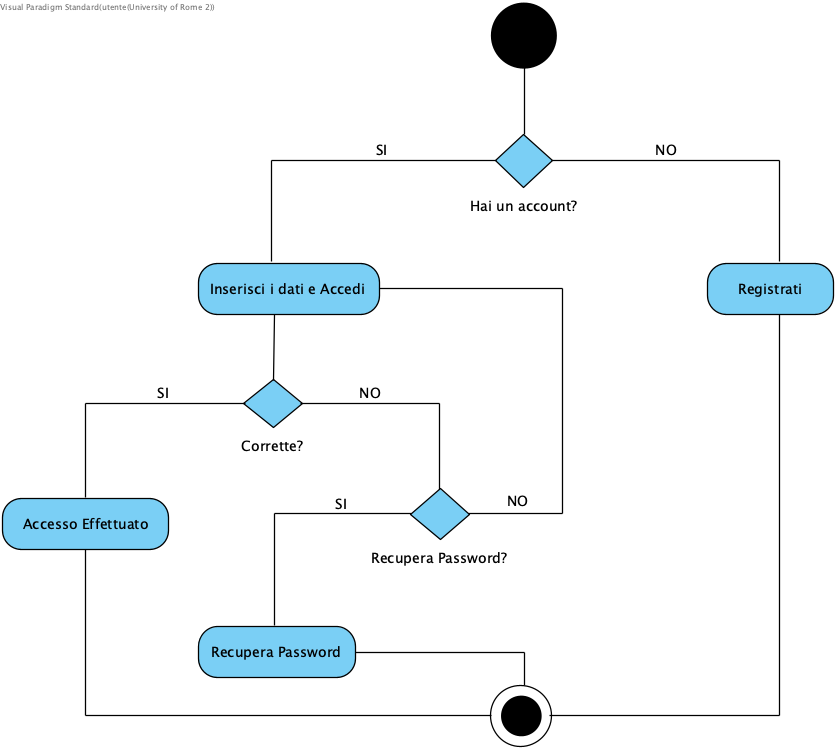
\includegraphics[width=0.5\textwidth]{Activity Diagram/Admin_Ente/Admin_Ente_(Autenticazione).png}
    \caption{}
    \label{fig:admin_auth}
\end{figure}
\noindent
Una volta effettuato l'accesso, l'Admin accede al Pannello di Mobilità. \\ Come illustrato in Figura \ref{fig:admin_pannello}, da questo snodo centrale l'utente può diramarsi in quattro attività principali: la gestione delle corse, della flotta, delle tariffe e dello staff. Ogni operazione prevede una fase di salvataggio e la possibilità di tornare al pannello principale per avviare una nuova attività.
\begin{figure}[H]
    \centering
    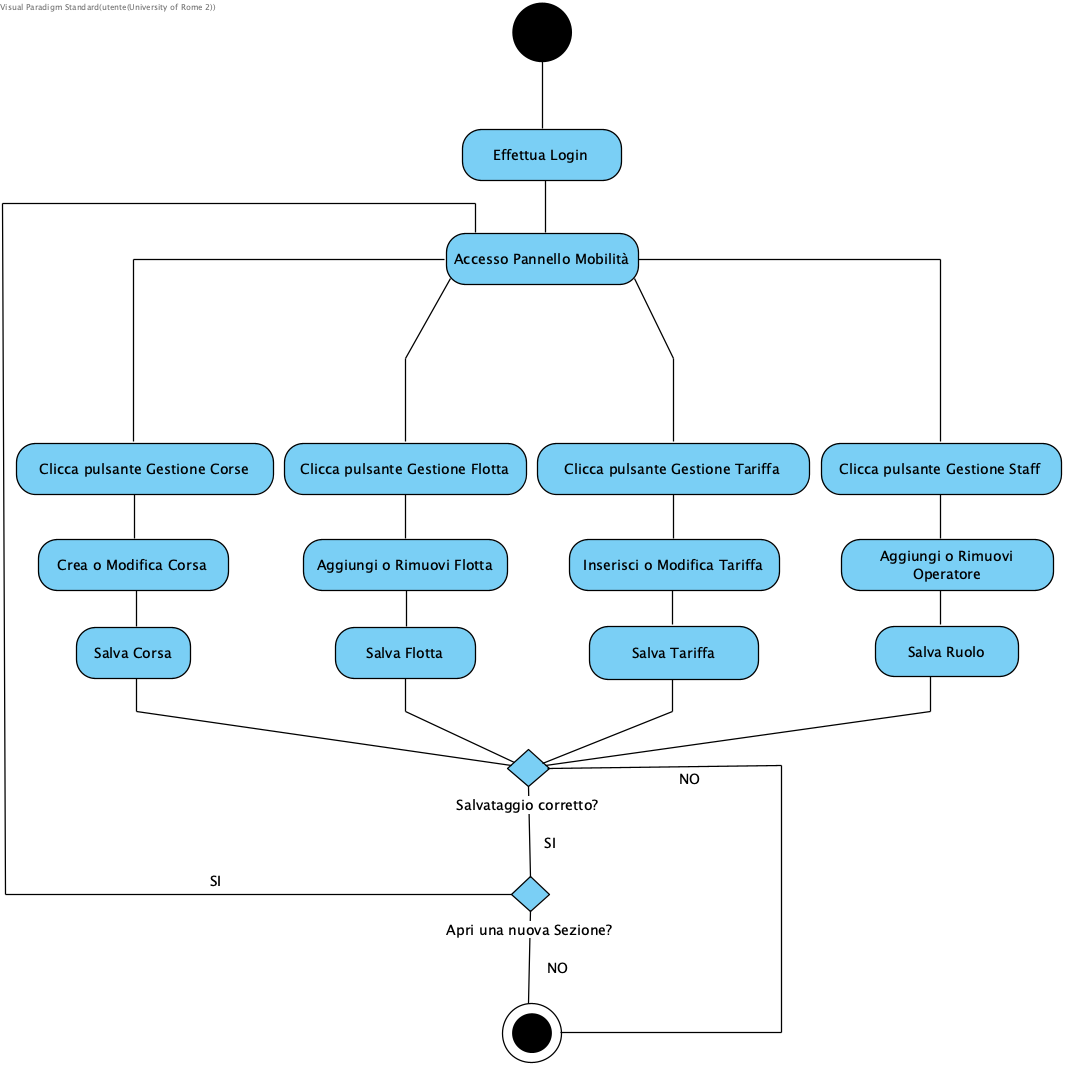
\includegraphics[width=0.5\textwidth]{Activity Diagram/Admin_Ente/Admin_Ente_(Gestione_Pannello_Mobilità).png}
    \caption{}
    \label{fig:admin_pannello}
\end{figure}
\newpage
% SEZIONE OPERATORE
\subsection*{Azioni dell'Operatore}
Un altro attore chiave della componente gestionale e operativa sul campo è l'Operatore, il quale interagisce con la piattaforma per le proprie mansioni quotidiane. Il suo flusso di autenticazione segue la logica standard del sistema (Figura \ref{fig:op_auth}).
\begin{figure}[H]
    \centering
    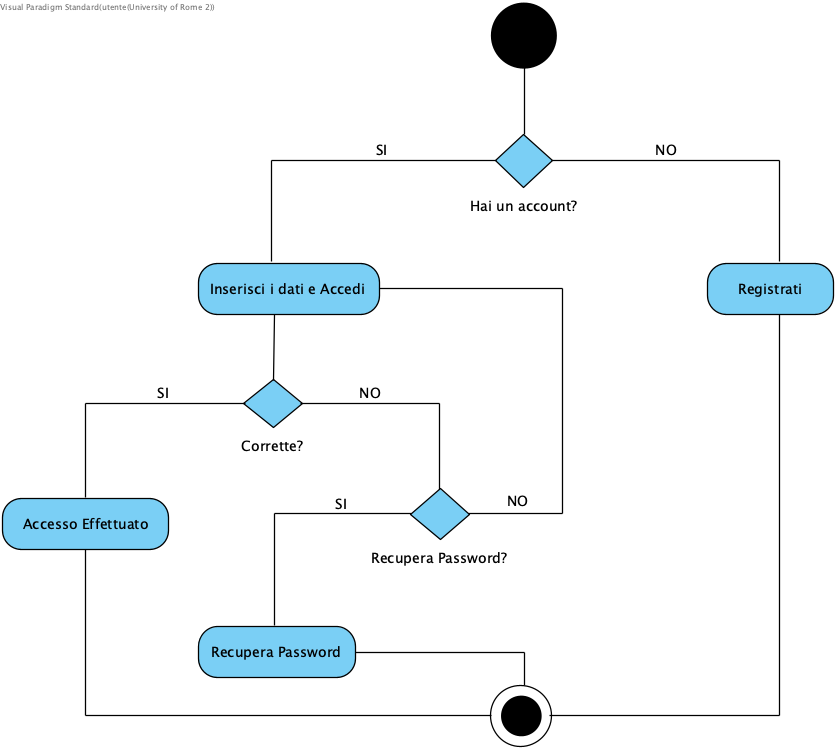
\includegraphics[width=0.5\textwidth]{Activity Diagram/Operatore/Operatore_(Autenticazione).png}
    \caption{}
    \label{fig:op_auth}
\end{figure}
\noindent
Nel contesto dei servizi di trasporto a chiamata (DRT), l'operatore riceve notifiche per nuove corse. Come vediamo in Figura \ref{fig:op_drt} vi è una semplice diramazione logica tra l'accettazione o il rifiuto della chiamata da parte dell'autista.
\begin{figure}[H]
    \centering
    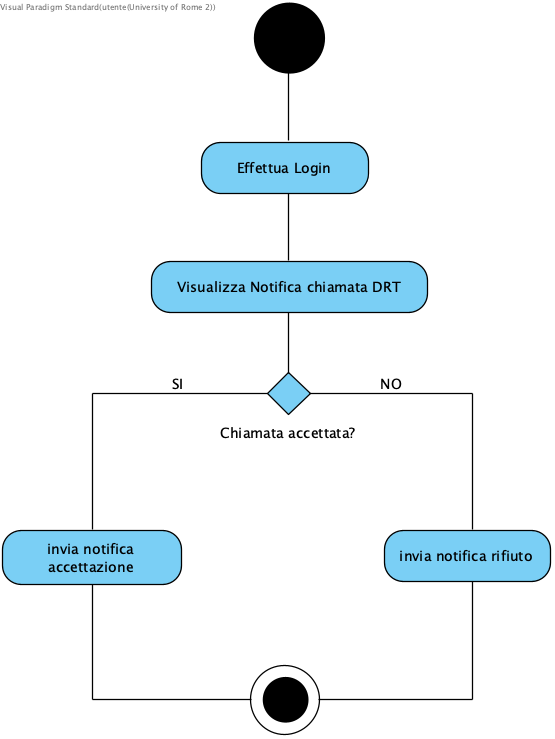
\includegraphics[width=0.3\textwidth]{Activity Diagram/Operatore/Operatore_(Gestione corse_DRT).png}
    \caption{}
    \label{fig:op_drt}
\end{figure}
\noindent
Una delle azioni più importanti dell'Operatore è quella di mantenere aggiornato lo stato del servizio. L'Activity Diagram in Figura \ref{fig:op_stato} mostra il processo ciclico di inserimento e caricamento dei dati aggiornati nell'area di servizio.
\begin{figure}[H]
    \centering
    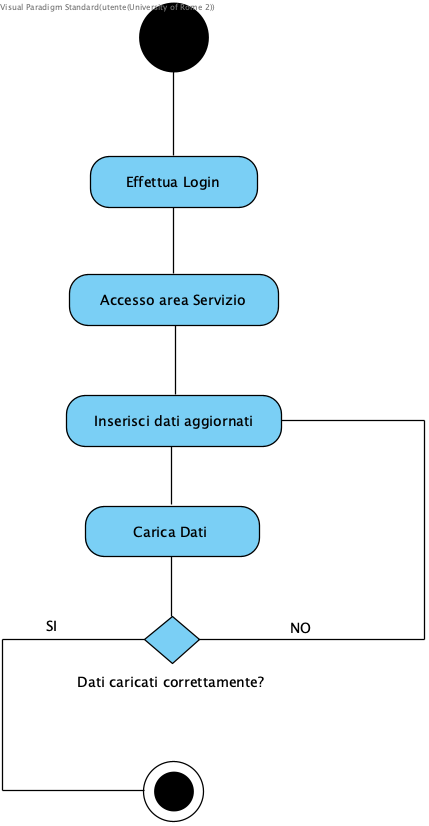
\includegraphics[width=0.3\textwidth]{Activity Diagram/Operatore/Operatore_(Stato_Servizio).png}
    \caption{}
    \label{fig:op_stato}
\end{figure}
\noindent
L'ultima azione, non per importanza, è la verifica dei titoli di viaggio. Come si evince dalla Figura \ref{fig:op_verifica}, l'operatore scannerizza il QRCode del biglietto. Se la lettura fallisce o il codice non è valido visivamente, il sistema offre un flusso alternativo permettendo l'inserimento manuale del codice.
\begin{figure}[H]
    \centering
    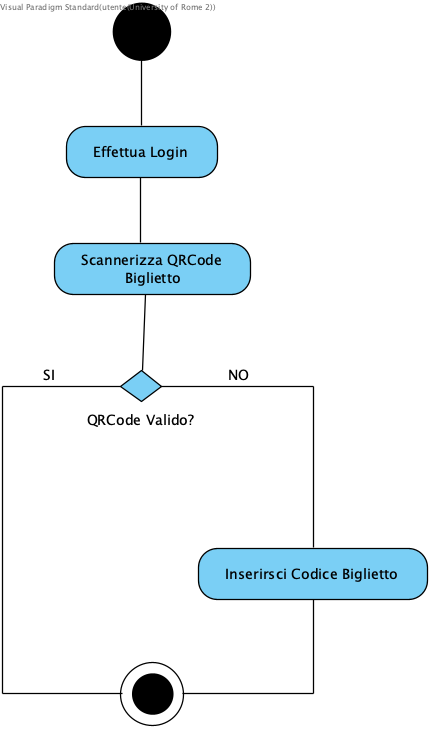
\includegraphics[width=0.3\textwidth]{Activity Diagram/Operatore/Operatore_(Verifica_Prenotazioni).png}
    \caption{}
    \label{fig:op_verifica}
\end{figure}
\newpage
% SEZIONE FUNZIONARIO COMUNALE
\subsection*{Azioni del Funzionario Comunale}
L'ultima figura che gestisce, stavolta dal punto di vista istituzionale, il software è il  Funzionario Comunale. Quest'ultimo ha un ruolo legato alla gestione degli avvisi e della viabilità cittadina. Il flusso parte regolarmente con l'autenticazione al portale (Figura \ref{fig:funz_auth}).
\begin{figure}[H]
    \centering
    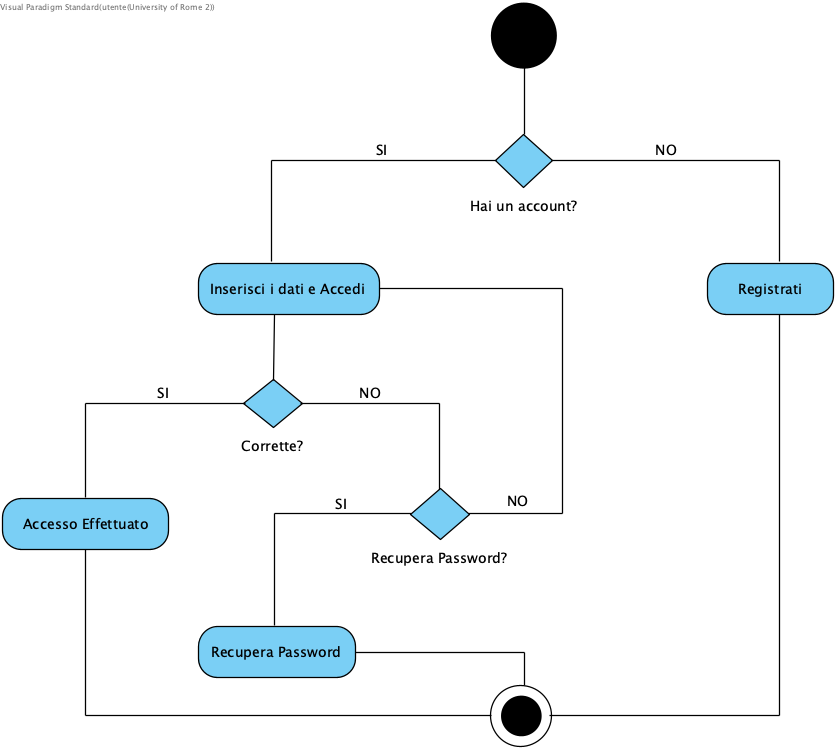
\includegraphics[width=0.5\textwidth]{Activity Diagram/Funzionario_Comunale/Funzionario_Comunale_(Autenticazione).png}
    \caption{}
    \label{fig:funz_auth}
\end{figure}
\noindent
Il funzionario ha accesso alla sezione Avvisi, dove può compiere diverse operazioni cruciali per la viabilità. La prima è la gestione delle ordinanze (Figura \ref{fig:funz_ordinanze}), che prevede il caricamento del documento e la verifica del corretto inserimento a sistema.\\
Un'altra operazione fondamentale è la comunicazione con altri enti. Come visibile in Figura \ref{fig:funz_notifica}, il funzionario può selezionare un avviso personale, scegliere l'ente destinatario, comporre un messaggio e inviarlo, con un controllo sull'esito della trasmissione.
\begin{figure}[H]
    \centering
    \begin{minipage}{0.2\textwidth}
        \centering
        \includegraphics[width=\textwidth]{"Activity Diagram/Funzionario_Comunale/Funzionario_Comunale_(Gestisce_Ordinanze).png"}
        \caption{}
        \label{fig:funz_ordinanze}
    \end{minipage}
    \hspace{3cm} 
    \begin{minipage}{0.2\textwidth}
        \centering
        \includegraphics[width=\textwidth]{"Activity Diagram/Funzionario_Comunale/Funzionario_Comunale_(Notifica_Enti).png"}
        \caption{}
        \label{fig:funz_notifica}
    \end{minipage}
\end{figure}
\noindent
Infine, per minimizzare l'impatto sul traffico durante gli eventi paesani, il funzionario può suggerire percorsi alternativi. Il diagramma in Figura \ref{fig:funz_percorsi} illustra l'inserimento dei dati relativi all'evento e il caricamento dei tracciati alternativi a sistema.
\begin{figure}[H]
    \centering
    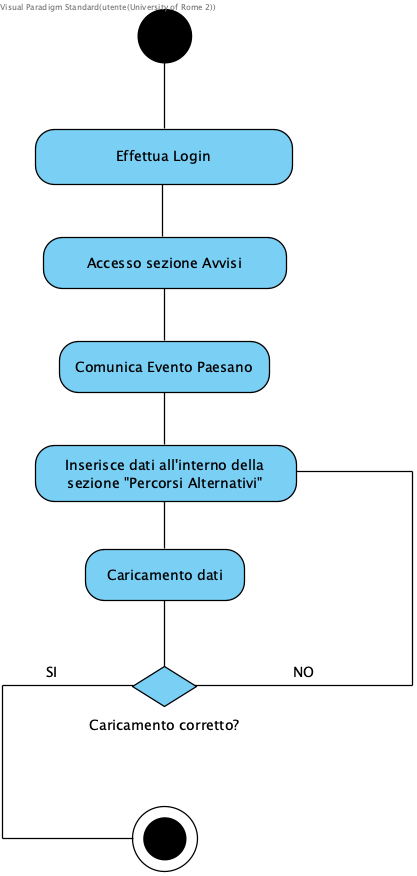
\includegraphics[width=0.4\textwidth]{Activity Diagram/Funzionario_Comunale/Funzionario_Comunale_(Suggerimento_Percorsi).png}
    \caption{}
    \label{fig:funz_percorsi}
\end{figure}
\newpage
% SEZIONE PAGAMENTI E RIMBORSI
\subsection*{Azioni del Payment}
Infine, per garantire la robustezza logica dell'intera applicazione, ho studiato i flussi relativi al modulo delle transazioni finanziarie. A differenza dei precedenti, questi diagrammi coinvolgono attivamente il backend e sistemi di terze parti (modellati tramite le \textit{partitions}). \\
La Figura \ref{fig:pay_elaborazione} mostra il processo di elaborazione dei pagamenti: il sistema riceve e controlla il formato dei dati; in caso di esito positivo, richiede l'autorizzazione a un modulo esterno o ente bancario e, all'arrivo della risposta di approvazione, aggiorna il database ed emette la ricevuta.
\begin{figure}[H]
    \centering
    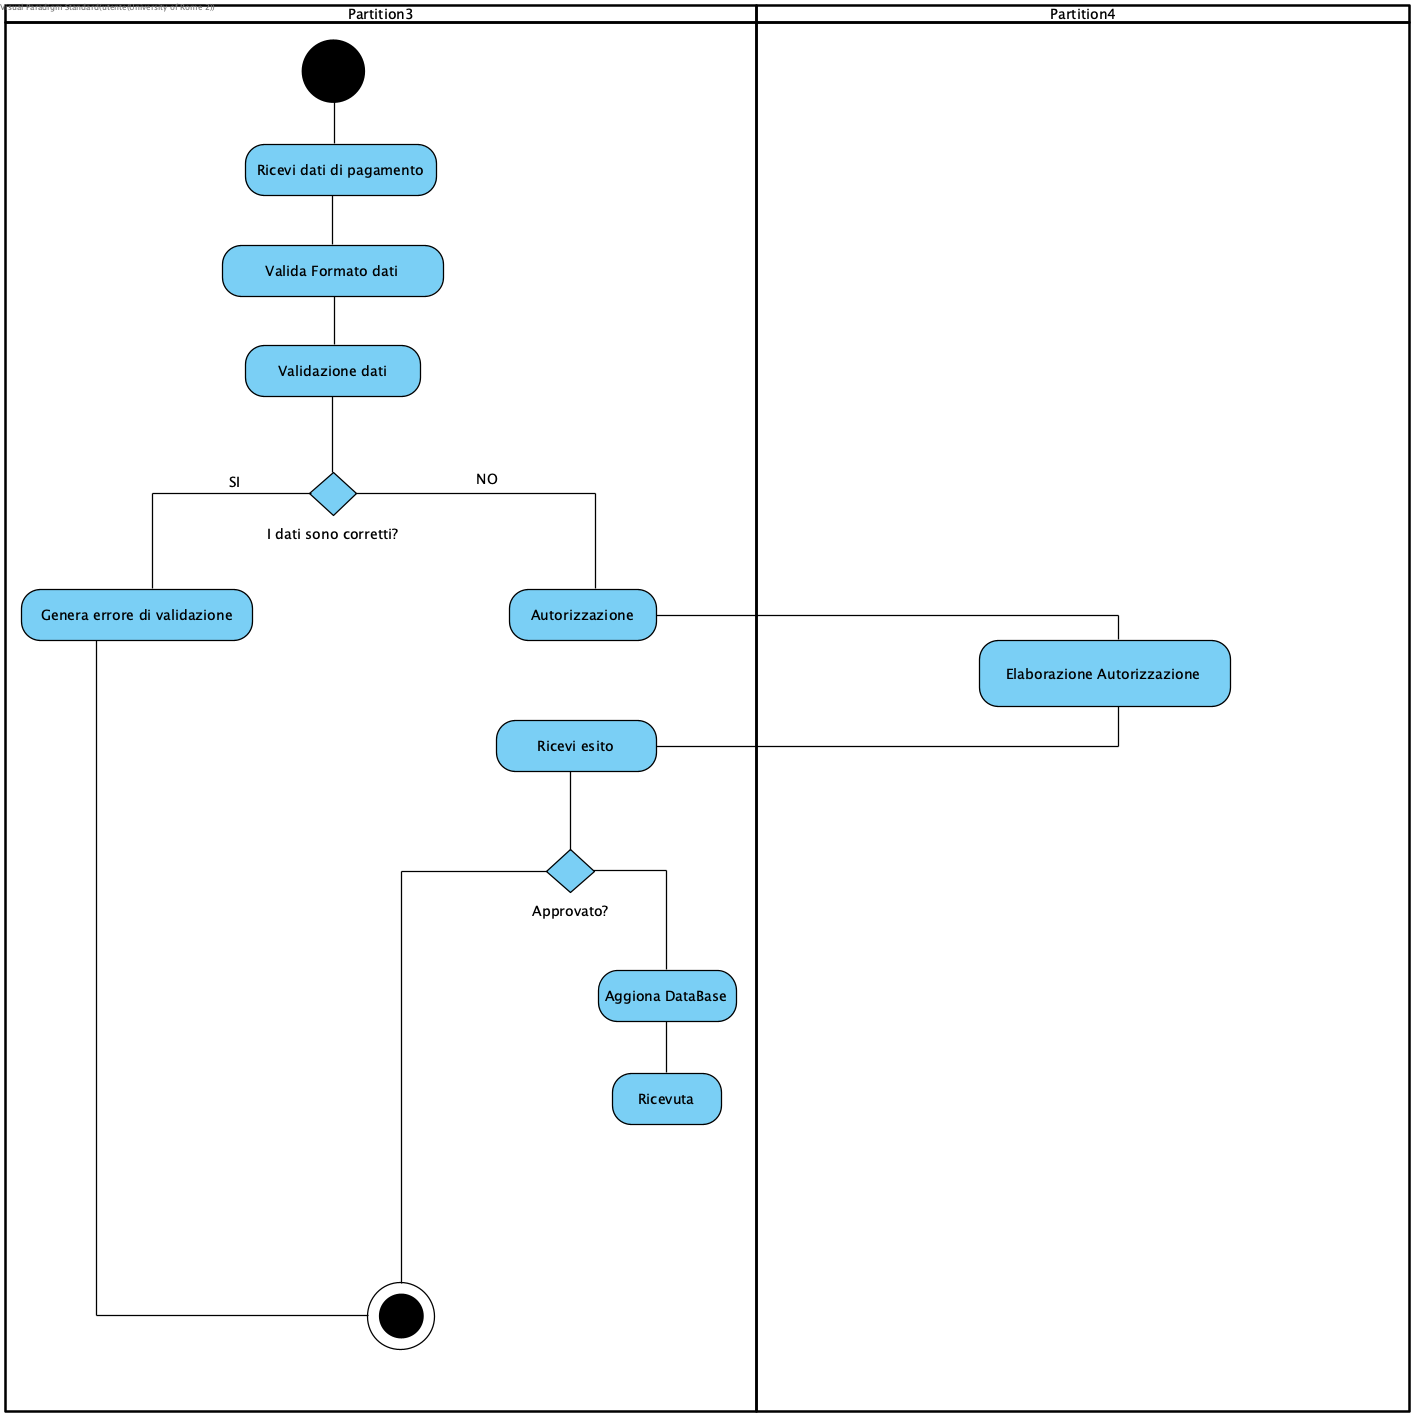
\includegraphics[width=0.4\textwidth]{Activity Diagram/Payment/Payment_(Elaborazione_Pagamenti).png}
    \caption{}
    \label{fig:pay_elaborazione}
\end{figure}
\noindent
Parallelamente, anche la gestione dei rimborsi (Figura \ref{fig:pay_rimborsi}) segue un iter di validazione rigoroso e cross-partition. A seguito di una richiesta, il sistema recupera la transazione, verifica i criteri di idoneità per il reso e, in caso positivo, elabora lo storno.
\begin{figure}[H]
    \centering
    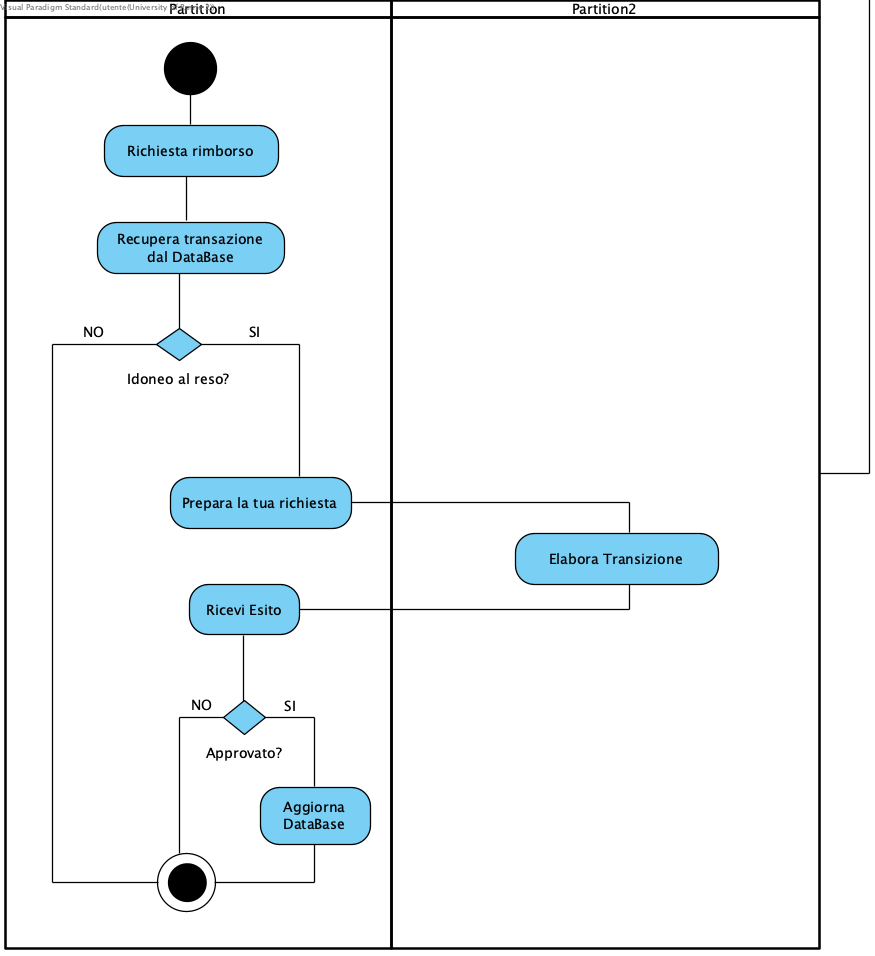
\includegraphics[width=0.4\textwidth]{Activity Diagram/Payment/Payment_(Gestione_RImborsi).png}
    \caption{}
    \label{fig:pay_rimborsi}
\end{figure}